\documentclass[]{standalone}

\usepackage{amsmath}
\usepackage{amsfonts}
\usepackage{amssymb}
\usepackage{graphicx}
\usepackage{tikz}
\usepackage{import}
\usepackage[subpreambles=true]{standalone}

\usepackage{tikz}
\usepackage{tikz-3dplot}


\usetikzlibrary{positioning}
\usetikzlibrary{decorations.markings}

\begin{document}


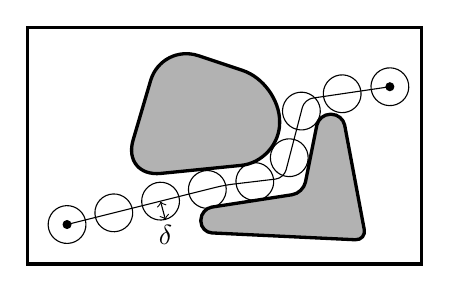
\begin{tikzpicture}[scale=1]

    \useasboundingbox (0,0) rectangle (5,3);
    
    \coordinate (obs1) at (2.4,2.1);
    \coordinate (obs2) at (3.7,0.65);
    
    \path[draw, very thick, rounded corners=14pt, fill=black!30] (obs1) node[shift={(-0.15,-0.25)}, transparent]{$\mathcal{C}_\mathrm{obs}$} ++(-1.2,-1) -- ++(2,0.2) -- ++(0,1) -- ++(-1.5,0.5) -- cycle;
    \path[draw, very thick, rounded corners=4pt, fill=black!30] (obs2) ++(-1.5,-0.25) -- ++(0,0.3) -- ++(1.3,0.2) -- ++(0.2,1) -- ++(0.3,0) -- ++(0.3,-1.6) -- cycle;
    
    % draw the bounding box
    \path[draw, very thick] (0,0) -- (5,0) -- (5,3) -- (0,3) -- cycle;
    
    % draw the connection radius
    % \begin{scope}
    %     \clip (0,0) rectangle (5,3);
    %     \path[draw, thick, dashed, fill=gray, fill opacity=0.2] (n7) circle (\radius);
    % \end{scope}
    
    
    \coordinate (init1) at (0.5,0.5);
    \coordinate (goal1) at (4.6,2.25);
    
    \path[draw, fill] (init1) circle (0.05);
    \path[draw, fill] (goal1) circle (0.05);
    \path[draw, rounded corners=3pt, decoration={
        markings,
        mark=
            between positions 0 and 1 step 0.125
            with {
                \path[draw] (0,0) circle (0.24);
            }
        }, postaction={decorate}] (init1) -- ++(2.0,0.50) -- ++(0.755, 0.09) -- ++(0.26,1.0) -- (goal1);
    
    \path[draw, <->] (1.75,0.56) node [below, shift={(0,0.05)}] {$\delta$} --  ++({cos(105)*0.24}, {sin(105)*0.24});
    
\end{tikzpicture}
\end{document}